\documentclass[12pt]{article}
\usepackage[english]{babel}
\usepackage{float}
\usepackage[margin=1in]{geometry}
\usepackage{graphicx}
%\usepackage[toc,page]{appendix}
\graphicspath{ {./img/} }
\newcommand{\rpm}{\raisebox{.2ex}{$\scriptstyle\pm$}} 
\usepackage{listings}
\usepackage{xcolor}
\usepackage{indentfirst}
\usepackage{caption}
\usepackage[final]{pdfpages}
\usepackage{amsmath}
\usepackage[normalem]{ulem}



\begin{document}

\title{Joe Phaneuf \\ Computer Vision 16-720 Spring 2018 Homework 5 \\ Apr. 8, 2018 }
\date{}
\author{}
\maketitle

\newpage


%\stepcounter{section}
%%%%%%%%%%%%%%%%%%%%%%%%%%%%%%%%%%%%%%%%%%%%%%%%%%%%%%%%%%%%%%%%%%%%%%%%%%%%%%%%
%%%%%%%%%%%%%%%%%%%%%%%%%%%%%%%%%%%%%%%%%%%%%%%%%%%%%%%%%%%%%%%%%%%%%%%%%%%%%%%%
\section{Q1}
\subsection{Q1.1}
Fundamental matrix F is defined for points $p1$ in image plane 1 and $p2$ in image plane 2 such that:  
$p2^{T} F p1 = 0$  
  
if $p1$ and $p2$ are at normalized image plane coordinates (0,0) , then in a homogeneous coordinate system  
$ p1 = p2 = \begin{bmatrix} 0 \\ 0 \\ 1 \end{bmatrix}$   
  
And consequently  

$$
p2^{T}
\begin{bmatrix}
f_{11} & f_{12} & f_{13} \\
f_{21} & f_{22} & f_{23} \\
f_{31} & f_{32} & f_{33}
\end{bmatrix}
p1
=
p2^{T}
\begin{bmatrix}
f_{13} \\
f_{23} \\
f_{33}
\end{bmatrix}
=
f_{33}
=0
$$

\newpage
\subsection{Q1.2}
Consider points $p1$ and $p2$ in image plane 1 and image plane 2, where cameras 1 and 2 are offset by translation $t$ and rotation $R$.  
  
$p2 = R ( p1 - t)$  
  
$(p1 - t ) ( t \times p1 ) = 0$  
  
$(p2^{T} R ) ( t \times P1 ) = 0$  
  
$p2^{T} R ) ( \begin{bmatrix} t \end{bmatrix}_{x} p1 ) = 0$

In the case that the cameras are offset by a pure translation along the x axis:   
  
$R = I , t = \begin{bmatrix} t_{x} \\ 0 \\ 0 \end{bmatrix}$  
  
$p2^{T} \begin{bmatrix} t \end{bmatrix}_{x} p1 = 0$
  
$$
E =
\begin{bmatrix} t \end{bmatrix}_{x}  = 
\begin{bmatrix} 0&0&0 \\ 0&0&-t_{x} \\ 0&t_{x}&0 \end{bmatrix}
$$

So epipolar line $l'$ can be found as :
  
$l' = E p1$

Looking at $E$ , the 1st column is all zeros , so $l'$ will have zero x component, thereby describing an epipolar line parallel to the x axis.

\newpage
\subsection{Q1.3}
Given rotation and translation measurements $R_{i}$ and $t_{i}$ at time step $i$ relative to some world or initialization frame , the relative rotation and translation between frames $i$ and $i+1$ are: 
  
$R_{rel} = R_{i}^{T} R_{i+1}$ 
  
$t_{rel} = R_{i}^{T} ( t_{i+1} - t_{i} )$  
  
The translation is just a difference of vectors rotated into the ith frame , and the rotation can be thought of as 'undoing' the rotation at $i$ back to the world/initialization frame and then doing the rotation to $i+1$.
  
The essential matrix is simply $E = R_{rel} \begin{bmatrix}  t_{rel} \end{bmatrix}_{x}$
  
And the fundamental matrix is $F = K^{-T} E K^{-1}$ 

\newpage
\subsection{Q1.4}
For an object reflected in a mirror (assuming object is parallel to the mirror) , we can imagine a view of the reflection that matches the original object view by translating a virtual camera frame. The virtual camera frame will have to be mirrored, but that's ok.
Recall that the essential matrix is made up of rotations and translations:
$E = R \begin{bmatrix} t \end{bmatrix}_{x}$ 

Where $\begin{bmatrix} t \end{bmatrix}_{x}$ is skew symmetric. Since there are no rotations, R is an identity matrix, so the essential matrix is skew symmetric.

Without knowledge of the 3 dimensional environment, we can set up the situation for the fundamental matrix, resulting in two images of the original object related by a skew symmetric fundamental matrix.


\newpage
\section{Q2}
\subsection{Q2.1}
Given two sets of correspondences from slightly different images of a temple, a fundamental matrix was recovered, shown below:
$$
\begin{bmatrix}
0.00000133  &  0.0000142  &  -0.21667407 \\
0.00002237  & -0.00000042 &  0.00017299 \\
0.20739486  ^ -0.00387777 &   1.         
\end{bmatrix}
$$
The fundamental matrix was used calculate and dras epipolar lines on the second temple image, shown in Figure \ref{fig:fepipolar}.

\begin{figure}[H]
\centering
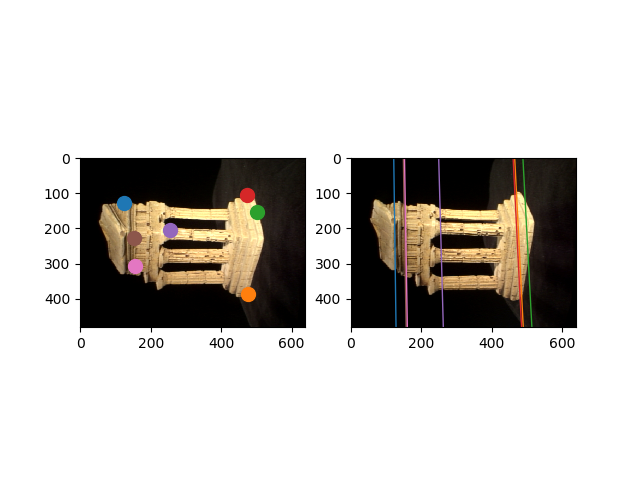
\includegraphics[page=1,width=0.75\textwidth]{q2_1}
\caption{ Epipolar lines  } 
\label{fig:fepipolar}
\end{figure}   

\newpage
\subsection{Q2.2}


The same process described in Q2.1 was applied with seven points using the seven point algorithm. The resulting fundamental matrix is :
$$
\begin{bmatrix}
-0.00000557  &  0.00004611  & -0.3589384 \\
0.00001358   & -0.00000301  &  0.01705569 \\
0.34818835   & -0.02150019  &  1.        
\end{bmatrix}
$$

The epipolar lines generated from F are shown in 

\begin{figure}[H]
\centering
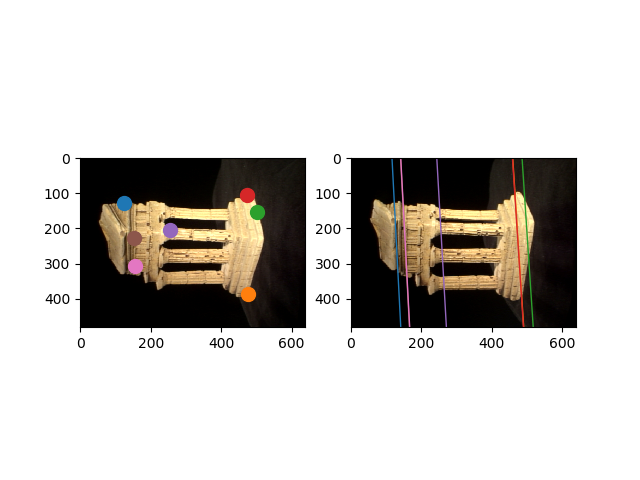
\includegraphics[page=1,width=0.75\textwidth]{q2_2}
\caption{ Epipolar lines using seven point algorithm } 
\label{fig:fepipolar7}
\end{figure}   

\newpage
\section{Q3}
\subsection{Q3.1}
Given the camera intrinsic matrices, the essential matrix was recovered from the fundamental matrix generated by the eight point algorithm.
The recovered fundamental matrix is:
$$
\begin{bmatrix}
0.00000133 & 0.0000142   & -0.21667407 \\
0.00002237 & -0.00000042 &  0.00017299 \\
0.20739486 & -0.00387777 &  1.        
\end{bmatrix}
$$

And the essential matrix calculated from that is:
$$
\begin{bmatrix}
29.02600051   &  310.85741019 & -3051.50532873
489.65276601  &  -9.28232229  & 98.3519351
3059.47658236 &    4.49312778 &    1.       
\end{bmatrix}
$$

\newpage
\subsection{Q3.2}
With reasonable projection matrices in hand, we can estimate 3d points from point correspondences in two images.  This is done by solving 3d points that best fit the projection matrix and image points.
The image points and projection matrices can be related as follows:  
  
$$
AX = 0
$$
Where X contains 3d points , and A contains information about projection matrices and image points. Each set of correspondences results in 4 entries in A, which we will call Ai and define as follows:

$$
A_{i} = 
\begin{bmatrix}
y p_{3}^{T} - p_{2}^{T} \\
p_{1}^{T} - x p_{3}^{T} \\
\hat{y} \hat{p}_{3}^{T} - \hat{p}_{2}^{T} \\
\hat{p}_{1}^{T} - \hat{x} \hat{p}_{3}^{T} 
\end{bmatrix}
$$
  
Where $p_{n}^{T}$ is the nth row of projection matrix P.

\newpage
\subsection{Q3.3}
Possible solutions for the second camera view's extrinsic matrix were calculated, and evaluated by triangulation.
The final extrinsic matrix M2 is:
  
$$
\begin{bmatrix}
0.99942022& 0.03233587& 0.01065891& -0.03217808 \\
-0.03399003& 0.9657396& 0.25727747& -1.         \\
-0.00197444& -0.2574906& 0.96627879& 0.1603499
\end{bmatrix}
$$
  
With the corresponding projectin matrix C2:
$$
\begin{bmatrix}
1.51892159e+03& -2.86811081e+01& 3.08331208e+02& -4.46572073e-01 \\
-5.23528170e+01& 1.41005536e+03& 6.31124932e+02& -1.48631442e+03 \\
-1.97444107e-03& -2.57490600e-01& 9.66278786e-01& 1.60349901e-01 \\
\end{bmatrix}
$$
  
Total triangulation error for points in image 1 is: 366.692075881  
  
Total triangulation error for points in image 2 is: 358.641029195  
  
Total eror is : 733.384151762  
  

\end{document}
